\chapter{Arquitectura de la aplicación}
\label{cap:diseno}
Este capítulo presenta la arquitectura del sistema.
Describe el diseño del módulo de razonamiento y muestra los diagramas de clases correspondientes.
También se presentan brevemente el diseño de la interfaz de la aplicación con los patrones de diseño usados en la misma.

% PARA DISEÑO
%%Figura~\ref{fig:sistema} 
%muestra un esquema de la arquitectura del sistema.
%Se observa la base del sistema constituida por el marco de trabajo dividido en dos partes principales relacionadas: Estrategias y Juegos, que definen las interfaces que deben implementar las estrategias y los juegos que se quieran desarrollar.
%Este incluye también el entorno de usuario interactivo y otros componentes estándar para el dominio de los juegos en IA.
%
%Las distintas implementaciones de estrategias y juegos no forma parte del marco de trabajo, lo que permite ampliar el número de estrategias y juegos del sistema.
%
%

%La siguiente sección describe la arquitectura del módulo de razonamiento.

\section{Módulo de razonamiento}
\label{sec:arquitectura_modulo_razonamiento}
El módulo de razonamiento se ha dividido en tres módulos más pequeños: el módulo de los juegos, el de los jugadores o estrategias y el de los heurísticos.
Todos los módulos se encuentran relacionados mediante unas interfaces definidas.
A continuación se describen en detalle cada uno de estos módulos.

\subsection{Juegos}
\label{ssec:arquitectura_juegos}
En el capítulo~\ref{cap:juegos} se definió formalmente un juego como una clase de problemas de búsqueda que contiene: un estado inicial, una función sucesor, un test terminal y una función de utilidad o función objetivo.
Definiendo una interfaz adecuada se puede construir un módulo que permita implementar fácilmente cualquier juego del tipo considerado.

La figura~\ref{fig:diagramaclases_juegos} muestra el diagrama de clases del módulo de juegos junto con los dos juegos considerados (Conecta-K y Go).
Para simplificar el diagrama no se muestra la implementación de ambos juegos, sino únicamente la relación existente entre ellos y el módulo de juegos.

\begin{figure}[!p]
	\centering
	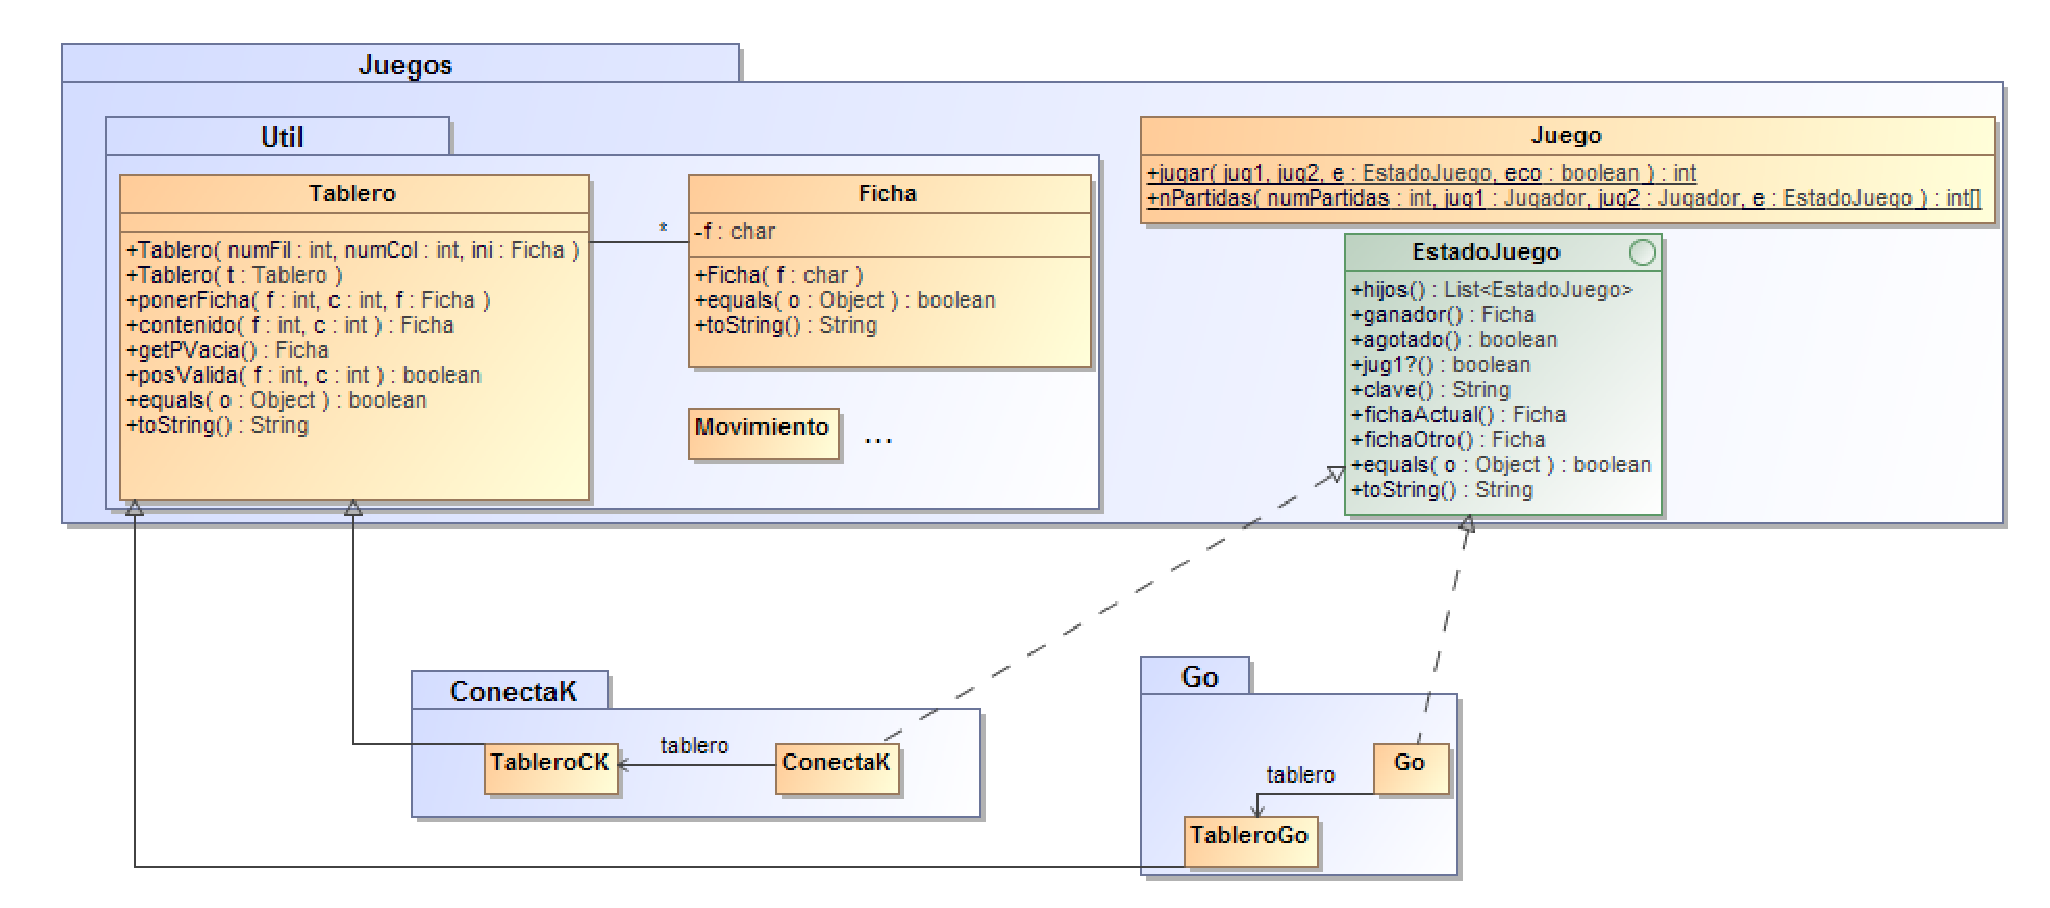
\includegraphics[scale=0.5,angle=90]{contenido/cap6/imagenes/diagramaclases_juegos.eps}
	\caption{Diagrama de clases de los juegos.}
	\label{fig:diagramaclases_juegos}
\end{figure}

El elemento principal del módulo de juegos es la interfaz \texttt{\textit{EstadoJuego}}, que proporciona una representación de los estados de un juego.
Se trata del elemento más importante de todo el módulo de razonamiento: cualquier juego debe implementar esta interfaz para representar sus estados.
La interfaz contiene una función sucesor (método \texttt{hijos}), un test terminal (\texttt{agotado}), y métodos que permiten indexar el estado en una posible estructura, conocer el ganador (si lo hay) y el jugador al que le toca jugar, comparar dos estados y proporcionar una descripción del estado.

Esta representación permite obtener el árbol de juegos a partir un estado gracias al método \texttt{hijos} que devuelve los sucesores inmediatos del estado actual.

Nótese que la interfaz no proporciona una función de utilidad para los estados terminales, ya que el método ganador sólo indica quién ha ganado.
El valor de utilidad al final de una partida se ha diseñado de manera independiente del juego: el método estático \texttt{jugar} de la clase \texttt{Juego} permite jugar una partida entre dos jugadores a partir de un estado inicial y devuelve el valor de utilidad obtenido (1 si gana el primer jugador, -1 si gana el segundo jugador y 0 en caso de empate).
Igualmente el método \texttt{nPartidas} juega un número determinado de partidas devolviendo los valores de utilidad de cada partida.

El módulo también proporciona un paquete de utilidades que ayuda a implementar los juegos como un tablero genérico, fichas o una representación de los movimientos.

El diagrama de la figura~\ref{fig:diagramaclases_juegos} sólo muestra en los paquetes \texttt{ConectaK} y \texttt{Go} las clases que representan a dichos juegos.
Estos paquetes son independientes del módulo de juegos y contienen otras clases como evaluadores heurísticos específicos para cada juego o jugadores dependientes del juego como el jugador humano.

\bigskip
El siguiente apartado muestra el diseño del módulo correspondiente a las estrategias.

\subsection{Estrategias}
\label{ssec:arquitectura_estrategias}
El módulo de estrategias se muestra en el diagrama de la figura~\ref{fig:diagramaclases_estrategias}.

\begin{figure}[!p]
	\centering
	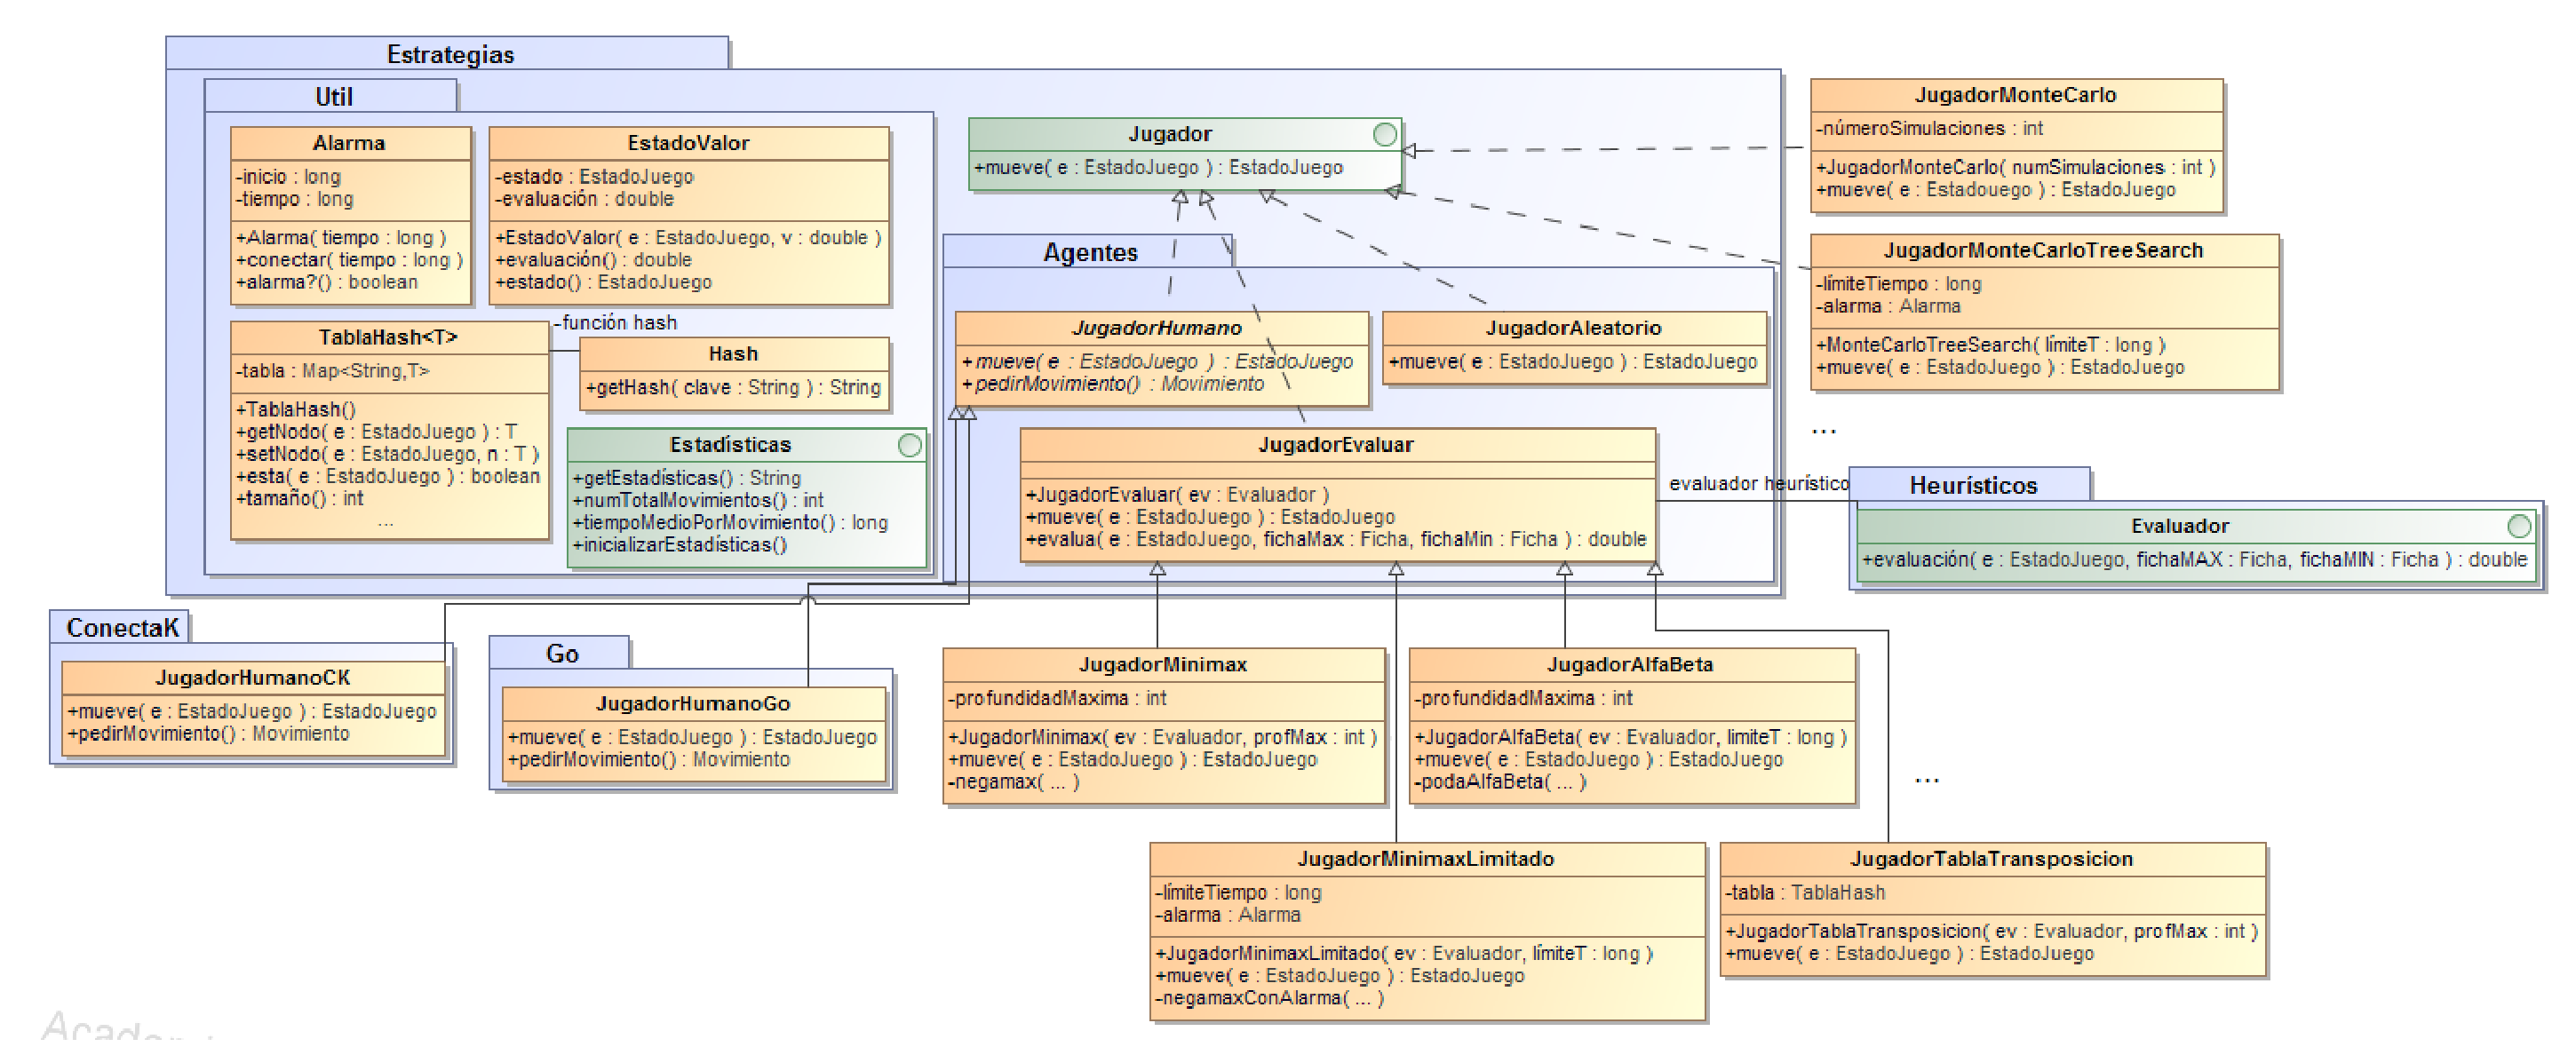
\includegraphics[scale=0.4,angle=90]{contenido/cap6/imagenes/diagramaclases_estrategias.eps}
	\caption{Diagrama de clases de las estrategias.}
	\label{fig:diagramaclases_estrategias}
\end{figure}

Toda clase que represente un agente jugador debe implementar la interfaz \texttt{\textit{Jugador}}.
Esta interfaz solamente tiene un método (\texttt{mueve}) que devuelve el estado resultante de que el jugador mueva en el estado actual dado.

El \texttt{JugadorAleatorio} implementa esta interfaz de forma general lo que le permite jugar a cualquier tipo de juego.
No ocurre lo mismo con el \texttt{JugadorHumano}, que necesita pedir el movimiento a realizar mediante un dispositivo de entrada, de ahí que se trate de una clase abstracta.
Cada juego debe implementar su propio jugador humano.

El \texttt{JugadorEvaluar} necesita de un evaluador heurístico que proporciona la evaluación de los estados; toda estrategia que necesite de un heurístico se considera una especialización de este jugador.
El resto de jugadores no forman parte del paquete \texttt{Estrategias} porque cada jugador puede implementar su estrategia de forma diferente, por ejemplo, la estrategia minimax se puede implementar siguiendo la definición \ref{eq:minimax} o mediante el algoritmo negamax (\ref{sssec:negamax}).
En el diagrama, por simplicidad, no aparecen todos las estrategias desarrolladas.

También se proporciona un paquete de utilidades para las estrategias que necesiten de una alarma de tiempo, una tabla hash o una función hash\footnote{La función hash implementada realiza una codificación mediante el algoritmo de reducción criptográfico \textit{MD5}\citeref{rfc1321}.}.
Para simplificar el diagrama tampoco se muestran explícitamente las asociaciones entre los jugadores y las utilidades usadas por cada uno.
Destaca la interfaz \texttt{\textit{Estadísticas}} que deberán implementar las estrategias que deseen proporciona sus propias estadísticas.

\bigskip
A continuación se detalla el módulo de los heurísticos.

\subsection{Heurísticos}
\label{ssec:arquitectura_heuristicos}
El módulo de heurísticos contiene las definiciones de los objetos evaluadores y permite entrenarlos mediante aprendizaje por refuerzo.
La figura~\ref{fig:diagramaclases_heuristicos} muestra en el diagrama de este módulo.

\begin{figure}[!p]
	\centering
	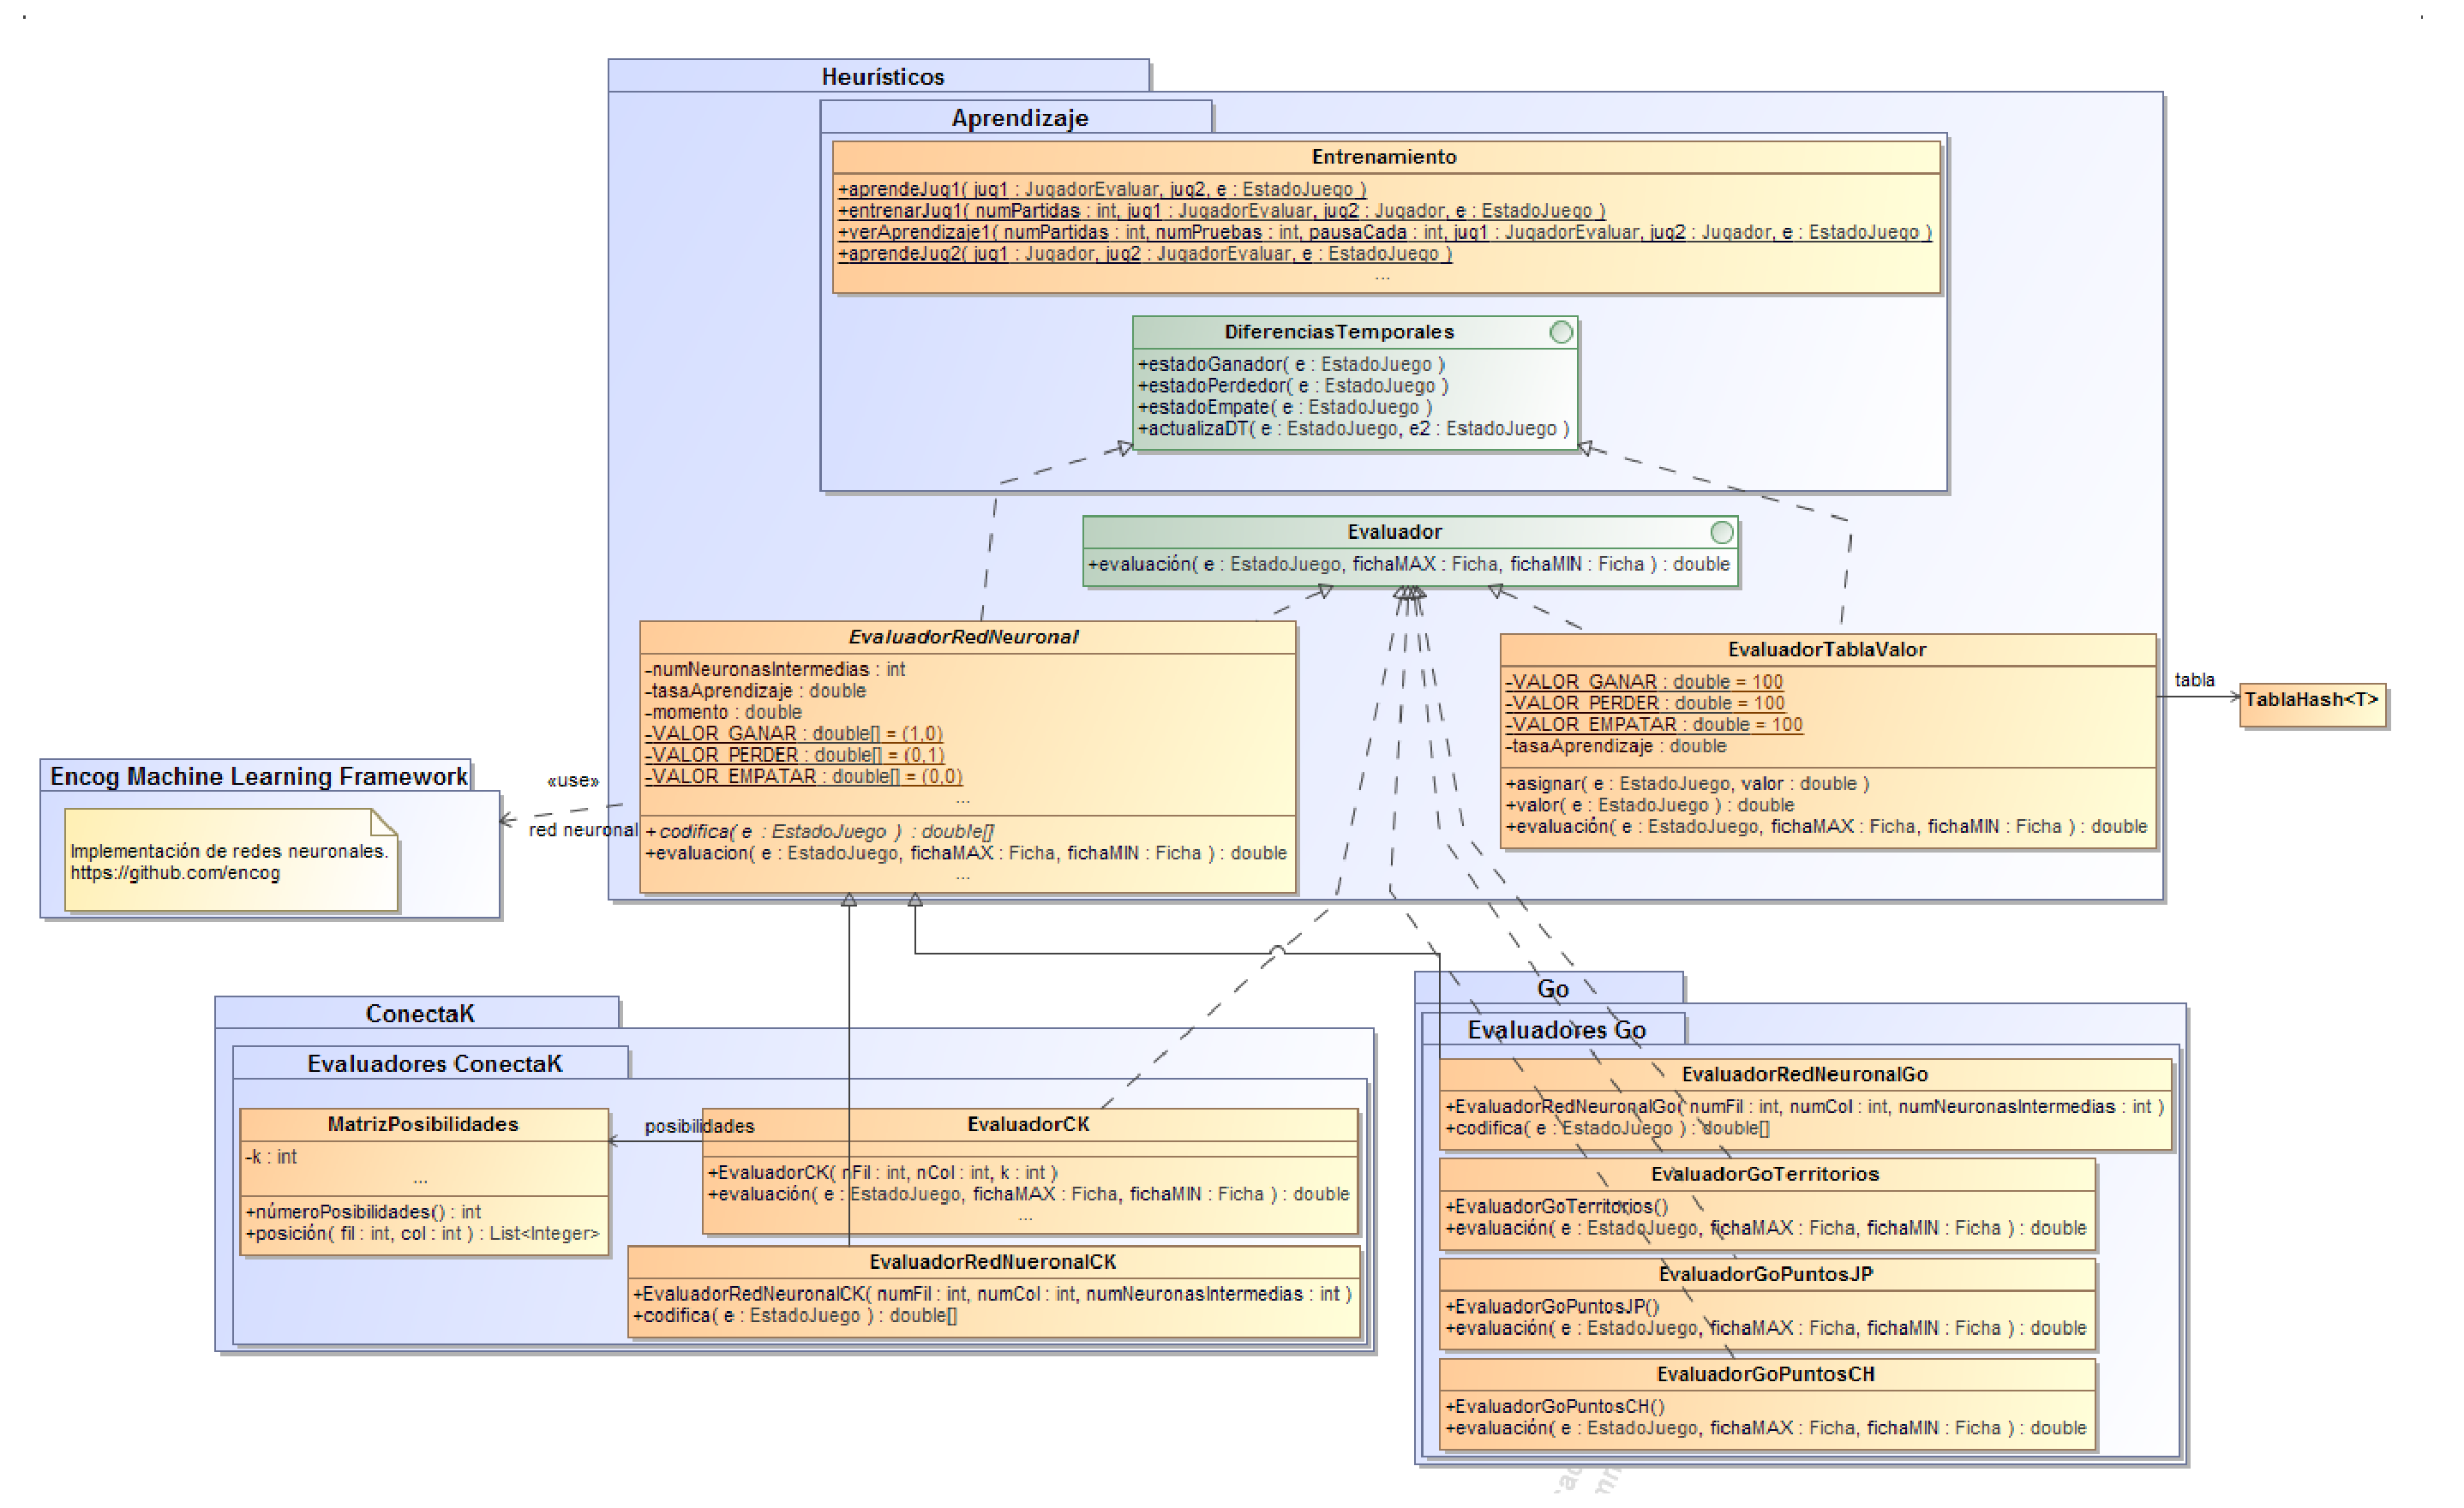
\includegraphics[scale=0.4,angle=90]{contenido/cap6/imagenes/diagramaclases_heuristicos.eps}
	\caption{Diagrama de clases de los heurísticos.}
	\label{fig:diagramaclases_heuristicos}
\end{figure}

La interfaz \texttt{\textit{Evaluador}} representa los objetos evaluadores heurísticos que proporcionan el valor de evaluación de un estado.
El juego que quiera proporcionar un heurístico para sus estados debe implementar esta interfaz siguiendo la definición de la función de evaluación heurística dada en~\ref{eq:heuristico}.

El módulo ofrece un paquete para definir evaluadores entrenables mediante aprendizaje por refuerzo; para ello los evaluadores deben implementar la interfaz \texttt{\textit{DiferenciasTemporales}}.
La clase \texttt{Entrenamiento} permite entrenar a los jugadores.
Debido a que los valores aprendidos por el evaluador son diferentes según se trate del primer jugador o del segundo, la clase proporciona métodos diferentes para entrenar al primer jugador, al segundo jugador o a ambos jugadores simultáneamente; para simplificar el diagrama, no se muestran todos estos métodos, pero sus cabecera son idénticas a las mostradas teniendo en cuenta que el jugador que entrena debe ser un \texttt{JugadorEvaluar} o una especialización del mismo.

El módulo también proporciona dos evaluadores: las tablas de valor y la red neuronal, ambos entrenables.
La red neuronal es una clase abstracta porque la función de codificación de los estados debe ser definida para cada juego.
Para la red neuronal se ha usado una implementación de libre distribución llamada \textit{Encog Machine Learning Framework} y que está disponible para varios lenguajes de programación~\citeref{encog}.

\bigskip
Los tres módulos juntos que se han presentado forman el marco de trabajo del proyecto.

\subsection{Marco de trabajo}
\label{ssec:marco_trabajo}
El marco de trabajo está compuesto por los tres módulos presentados en las secciones anteriores, concretamente los paquetes: \texttt{Juegos}, \texttt{Estrategias} y \texttt{Heurísticos}.

El marco de trabajo es una arquitectura especializada para el dominio de los juegos en IA; describe las interfaces, implementa algunos componentes y establece las reglas de interacción entre los componentes.
No se trata de una biblioteca de clases puesto que el marco de trabajo contiene abstracciones que pueden instanciar o invocar a las abstracciones del desarrollador que extienda el marco.

Los diagramas de las figuras \ref{fig:diagramaclases_juegos}, \ref{fig:diagramaclases_estrategias} y \ref{fig:diagramaclases_heuristicos} muestran también las extensiones del marco de trabajo, permitiendo extenderlo mediante herencia (extensión de caja blanca) o mediante composición (extensión de caja negra).

\bigskip
A continuación se describe la arquitectura de la aplicación interactiva que hace uso del módulo de razonamiento.

\section{Aplicación interactiva}
\label{sec:arquitectura_aplicacion_interactiva}
La aplicación interactiva es en realidad una interfaz de usuario para el módulo de razonamiento del sistema, que da acceso a toda su funcionalidad de forma fácil y atractiva.

Para diseñar la aplicación se ha seguido en todo momento el principio de integridad conceptual, por el cual los patrones generales de diseño del sistema se reflejan en cada parte del mismo. Un ejemplo es el sistema de ayuda de la aplicación, cuyo patrón se puede apreciar en cada parte de la interfaz.
Lo mismo ocurre con el patrón \textit{Modelo-Vista-Controlador} (\textit{MVC}) aplicado independientemente a cada parte de la aplicación, aunque su uso no se refleje en la estructura global del sistema.

El diagrama de la figura~\ref{fig:diagramaclases_gui} muestra las clases e interfaces que facilitan la incorporación de los juegos, estrategias y heurísticos a la interfaz gráfica.

\begin{figure}[!p]
	\centering
	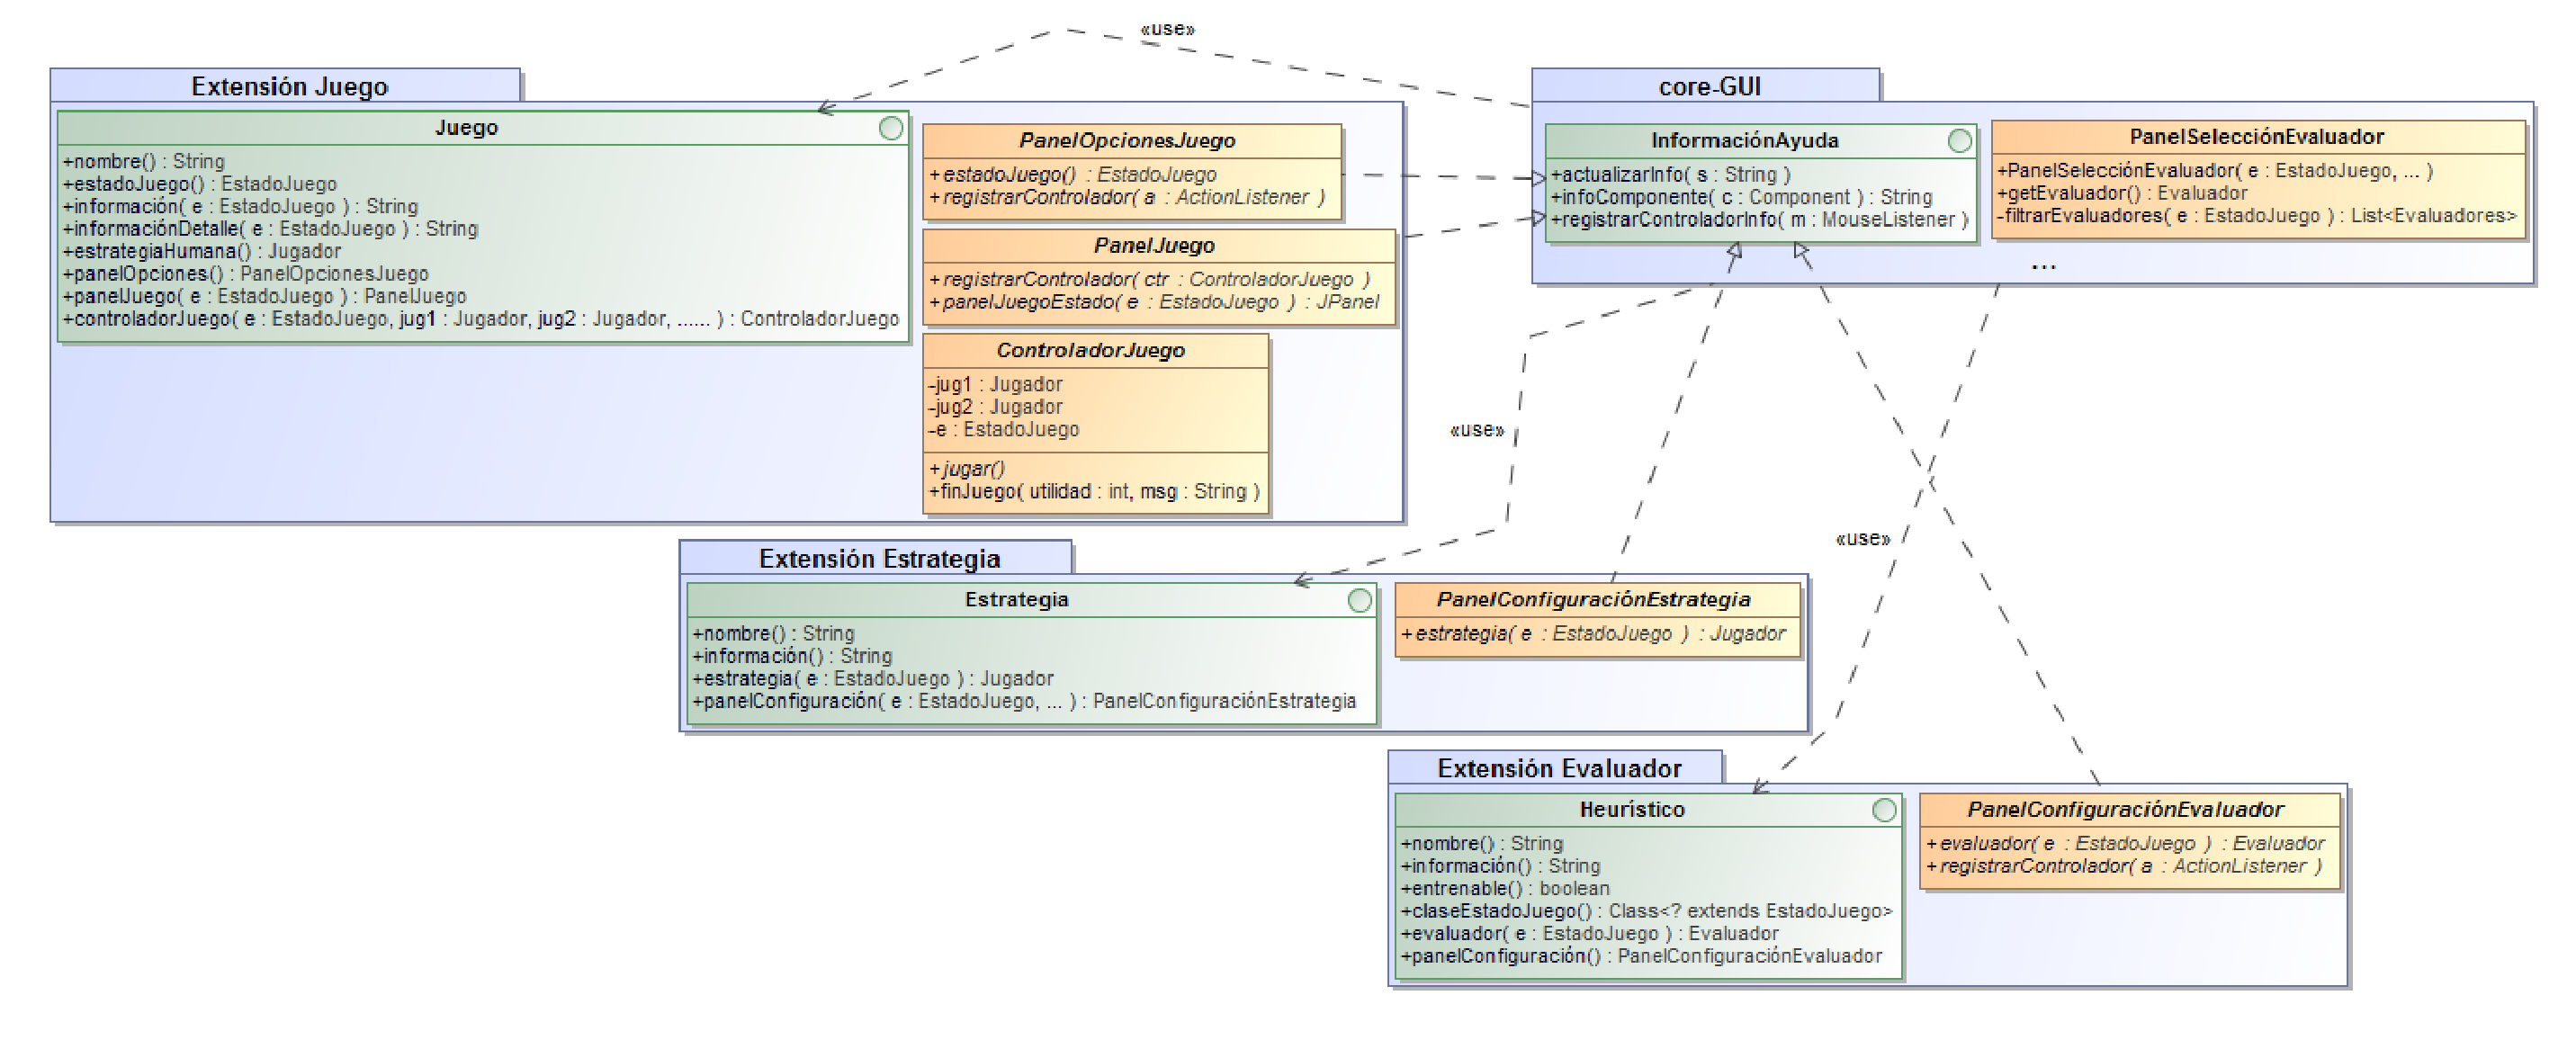
\includegraphics[scale=0.4,angle=90]{contenido/cap6/imagenes/diagramaclases_gui.eps}
	\caption{Diagrama de clases de las extensiones de la interfaz gráfica.}
	\label{fig:diagramaclases_gui}
\end{figure}

Todos los juegos, estrategias y heurísticos desarrollados se han incorporado a la interfaz de la aplicación interactiva siguiendo el esquema mostrado.
Cada elemento debe implementar su respectiva interfaz, lo que supone a su vez desarrollar los paneles de configuración adecuados, los controladores o el tablero para los juegos.

El núcleo de la interfaz gráfica consta de las vistas y los controladores necesarios para llevar a cabo los casos de uso de la aplicación, aunque estas clases no se muestran en el diagrama.

El sistema de información de ayuda está representado por la interfaz \texttt{\textit{InformaciónAyuda}}, que es implementada por cada componente visual de la interfaz gráfica (pantallas y paneles) usando el patrón de diseño \textit{Cadena de Mando} (\textit{Chain of Responsability}).
El usuario puede obtener información de ayuda sobre cualquier parte de la interfaz situándose sobre ella; la ayuda que se obtiene depende de la parte de la interfaz sobre la que solicita y de su contexto.

Por último, destacar que la aplicación se ha realizado íntegramente sobre tecnología \textit{Java} \citeref{java} en su versión 1.6; aunque el diseño propuesto permite desarrollar el entorno interactivo al completo en cualquier lenguaje de programación orientado a objetos.
La documentación en este proyecto es un aspecto clave, por lo que todo el código desarrollado se encuentra documentado en formato \textit{javadoc} para que cualquier alumno, profesor o investigador pueda hacer uso de él.

